\begin{chapterabstract}
  Histone H2AX is a histone variant found in almost all eukaryotes. It
  makes a central contribution to genome stability through its role in
  the signaling of DNA damage events and by acting as a foundation for
  the assembly of repair foci. The H2AX protein sequence is highly
  similar and in some cases overlapping with replication-dependent
  canonical H2A, yet the H2AX gene and protein structures exhibit a
  number of features specific to the role of this histone in DNA
  repair.  The most well known of these is a specific serine at the
  extreme C-terminus of H2AX which is phosphorylated by
  Phosphoinositide--3--Kinase-related protein Kinases (PIKKs) to
  generate the \textgamma H2AX mark. However, recent studies have
  demonstrated that phosphorylation, ubiquitylation and other
  post-translational modifications are also crucial for function. H2AX
  transcript properties suggest a capability to respond to damage
  events. Furthermore, the biochemical properties of H2AX protein
  within the nucleosome structure and its distribution within
  chromatin also point to features linked to its role in the DNA
  damage response. In particular, the theoretical inter-nucleosomal
  spacing of H2AX and the potential implications of amino acid
  residues distinguishing H2AX from canonical H2A in structure and
  dynamics are considered in detail. This review summarises current
  understanding of H2AX from a structure--function perspective.
\end{chapterabstract}

\section{Introduction}

Maintenance of the genome stability is of great importance to all
organisms because DNA damage can have serious biological implications
including genetic disorders and cancer \citep{PJM07}. One mechanism
for maintaining genome stability is to increase DNA repair
\citep{CLKWK98} and an important paradigm for DNA repair is the
mechanism for identifying and facilitating re-ligation of DNA Double
Strand Breaks (DSBs). DSBs are one of the most serious forms of DNA
damage because they involve loss of genetic continuity. They arise
from a variety of causes including not only the action of DNA damaging
agents but also normal functions such as meiosis and antibody class
switching. An important player in the DNA Damage Response (DDR) for
dealing with DSBs is the histone variant H2AX, which is an integral
component of the chromatin packaging of eukaryotic genomes.

\subsection{Chromatin Structure and Genome Stability}
Eukaryotic DNA is not dispersed randomly within the cell
nucleus. Instead, it is packaged into the chromatin structure which
compacts DNA and organises accessibility to the genome. This chromatin
packaging is hierarchical, based on the nucleosome as a fundamental
building block. The canonical nucleosome comprises two copies of each
core histone (H2A, H2B, H3 and H4) around which \SI{147}{\bp} of DNA is
wound in a superhelical spiral \citep{richmond-1kx5-19ansgtrom}. The nucleosomes are
connected by short DNA linkers to form repeating units which
subsequently arrange in a number of higher-order structural levels up
to condensed metaphase chromosomes.

Despite its modular structure, the arrangement of chromatin is not
static and must be ``remodeled'' during nuclear processes including
DNA repair. This remodeling is driven by two general mechanisms:
Firstly, molecules such as ATP-dependent remodelers and
chromatin-binding proteins can directly modify the
structure. Secondly, physiochemical properties of chromatin can be
modulated by post-translational modification or insertion of histone
variants to alter its stability \citep{controlling-double-helix,JA06}.

\subsection{H2AX and DNA repair}
H2AX and another histone variant, H2A.Z, were both identified in human
cells by their different migration compared to canonical H2A isoforms
on SDS and acetic acid--urea gels \citep{MHPW80}. In this separation,
H2AX and H2A.Z were two of four unidentified species arbitrarily
labeled T, W, X and Z\@. Subsequently, it was found that T and W were
the ubiquitylated forms of X and Z \citep{MHPW80}.
H2A.Y is an alternative name for macroH2A1. Although originally
labeled as H2A.X, the internal period (`\,.\,') separating the X has
fallen into disuse so the H2AX name is almost universally used in the
DNA repair field. In contrast, the internal period has historically
been retained in H2A.Z, whose major roles have been subsequently
associated with transcription \citep{JA06}.

A distinct function for H2AX was uncovered some 18 years after its
initial identification when human and mouse serine 139 was observed to
be rapidly phosphorylated in response to treatments that cause DSBs
\citep{EPR+98}. In structural nomenclature, the phosphorylation occurs
on the serine oxygen in the gamma position so the modified form is
widely referred to as \textgamma H2AX\@. This \textgamma H2AX
phosphoprotein is found to be rapidly concentrated around DSBs in
centers termed ``foci'' that can extend for a range of up to
\SI{2}{\mega\bp} away from the damage site \citep{EPR+99}.

The amino acid region surrounding serine 139 matches the consensus
recognition sequence for a set of PhosphoInositide--3--Kinase-related
protein Kinases (PIKKs) known to be central in the DNA damage response
from genetic studies in yeast \citep{JAD00}. The link between PIKKs
and \textgamma H2AX formation has been directly demonstrated by
biochemical inhibition using mutagenesis in yeast \citep{JAD00} and
wortmannin in higher cells \citep{TTP+00}.

\textgamma H2AX is a widely recognised participant in DSB repair and
is one of the earliest markers of damage \citep{DRP+03}. Other DNA
repair-related proteins subsequently congregate at the \textgamma H2AX
foci during the repair process. Although their recruitment to DSBs is
not completely dependent on H2AX phosphorylation, H2AX is an important
element in proper damage response foci formation by enhancing the
retention of repair factors after their initial recruitment
\citep{ACOF+03}.  H2AX$^{-/-}$ mice have moderate defects including
radiation sensitivity, growth retardation and immunodeficiency which
are consistent with deficiencies in DNA repair
\citep{ACSP+02,ACSD+03}.
Importantly, these phenotypes are only moderate and suggest redundancy
for the role of H2AX\@. Nevertheless, karyotypes of H2AX-deleted
genomes also reveal a high number of translocations and chromosome
rearrangements directly demonstrating increased genomic instability.

\section{Structural Properties of H2AX}
Based on the linkage between the early H2AX phosphorylation event and
the DDR, a large number of studies have focussed on \textgamma H2AX
and its subsequent interactions with the repair mechanism.
Less consideration has been given to the biochemical properties of
H2AX itself.

H2AX is one of a set of histone H2A proteins encoded in eukaryotic
genomes, the human genome holding 21 genes of H2A forms. The canonical
human H2A has two biochemically separable isoforms, H2A.1 and
H2A.2. No functional difference between those isoforms is known, and
the basis of their distinction appears to be dependent on residue 51
encoding, respectively, either a leucine or methionine despite further
heterogeneity within each isoform \citep{DBMC+06,Marzluff02}. Four
additional H2A variants with distinct functions are encoded in humans
and other higher eukaryotes: H2AX, H2A.Z, macroH2A1, macroH2A2,
H2A.F/Z and H2ABbd \citep{Marzluff02}.

\subsection{Definition of H2AX}
\label{subsec:h2ax-review:relation-H2A-H2AX}
The H2AX variant is principally defined by the capacity to accept
phosphorylation on a serine near the C-terminus through the activity
of PIKKs such as ATM, ATR and DNA-PK on the consensus motif
SQ[E/D]\textPhi (where \textPhi is a hydrophobic residue). The number
of residues separating this motif from the core histone fold region is
variable and has been claimed to correlate with the evolutionary
complexity of the organism \citep{CRDP+02}. For example, the spacing
of 29 residues between the end of the H2AX \textalpha 3 helix and the
phospho serine in \species{Saccharomyces cerevisiae} and
\species{Giardia lamblia} is 12 residues shorter than in humans and
mice.

In higher eukaryotes, H2AX is encoded as a separate histone variant of
H2A but in lower organisms such as \species{S.\ cerevisiae},
\species{G.\ lamblia} and certain protists, the distinguishing H2AX
features are merged into the canonical H2A \citep{HSM03,SJN06} so that
the canonical H2A also acts as the H2AX variant. In
\species{Drosophila melanogaster}, the H2AX feature is instead merged
with H2A.Z as a single variant, H2AvD, that is distinct from the
canonical H2A \citep{MCG02}.

Based on phylogenetic analysis, it has been suggested that H2AX
appeared multiple times in eukaryotes as an example of parallel
evolution \citep{HSM03}. However, the differences between metazoan
H2AX and canonical H2A sequences are few in number and this could be
confounding to phylogenetic algorithms. An alternative hypothesis is
that the H2AX function is ancestral and canonical H2A evolved from the
H2AX when complete phosphorylation became unnecessary or undesirable
as genomes expanded. This would explain the preeminence of the H2AX
variant in \species{G.\ lamblia} and \species{S.\ cerevisiae} compared
to the lower abundance in mammals.

It has remained something of a puzzle that no H2AX variant function is
identifiable in \species{Caenorhabditis elegans} \citep{HSM03} or some
protists \citep{SJN06}. A search of all predicted
\species{C.\ elegans} histones protein sequences reveals no PIKK
consensus motifs in the coding sequence or in any frame downstream of
the annotated stop codons for any of the core histone genes (data not
shown). However, the related \species{C.\ briggsae} genome contains
the motif SQDY within the \mbox{cpar-1} isoform of \mbox{CENP-A},
the centromeric \mbox{H3-like} histone. Alignment of seven known
\species{Caenorhabditis} \mbox{CENP-A} homologues shows that this
motif is quite conserved, with the sequence being SSDL in
\species{C.\ elegans} \mbox{cpar-1}
\frefp{fig:h2ax-review:celegans}. Although these do not strictly
conform to the classic PIKK recognition site sequence, non-canonical
sites are known to be recognised by them \citep{SYC+05}.

This potential merger of H2AX with \mbox{CENP-A} is interesting for
several reasons: Firstly, \species{C.\ elegans} utilises holocentric
chromosomes so \mbox{cpar-1} is thought to be distributed throughout
the genome \citep{MMH+05}. Secondly, \mbox{cpar-1} appears to be more
weakly expressed than the other \mbox{CENP-A} homologue in the
\species{C.\ elegans} genome, \mbox{hcp-3} \citep{MMH+05}, recalling
the H2AX/H2A ratio in human and mouse chromatin. Finally, the
SQDY/SSDL motif is located at small 3--4 residue insertion unique to
the core histone fold of \mbox{CENP-A} family proteins.
This insertion immediately abuts lysine 79 of canonical H3 which is
also implicated in the DDR
\frefp{fig:h2ax-review:celegans}\@. \mbox{CENP-A} family
proteins do not have lysine at the equivalent of position 79 of
canonical H3.

\begin{figure}
\centering

\includegraphics{h2ax-review/figs/Fig1}
\caption[Alignment of \species{Caenorhabditis} \mbox{CENP-A} homologues]%
        {Alignment of \species{Caenorhabditis} \mbox{CENP-A}
          homologues showing conservation of possible PIKK recognition
          site inserted within H3 structure. The major
          \species{C\@. elegans} \mbox{CENP-A} homologue
          (\mbox{hcp-3}) and a canonical H3 isoform (\mbox{his-2})
          with lysine 79 underlined are shown above.}
\label{fig:h2ax-review:celegans}
\end{figure}

\subsection{H2AX Gene}
Canonical histone genes in humans are spread over one large and two
small clusters named HIST1, HIST2 and HIST3. These are located at
6p21--p22, 1q21 and 1q42 respectively
\trefp{tab:h2ax-review:H2A-localisation}.
Canonical H2A is encoded by sixteen genes, twelve of which are located
in HIST1, three in HIST2 and one in HIST3. H2A variants are located
outside these histone clusters in the human genome, with the
H2AX--encoding gene H2AFX at 11q23.2--11q23.3 \citep{IZP+94}
\trefp{tab:h2ax-review:H2A-localisation}.
Histone variant gene names typically include the letter F for family.

\begin{table}
\centering
\caption[Localisation of all human canonical and variant H2A genes and
         proteins]%
        {Localisation of all human canonical and variant H2A genes and
          proteins (adapted from \citet{Marzluff02})}
\label{tab:h2ax-review:H2A-localisation}
\begin{tabular}{l l l l}
\toprule
Histone cluster & Gene & Protein & Locus  \\
\midrule
HIST1 & H2A A--E, G--M  & H2A.1           & 6p21--22\\
HIST2 & H2A A--C        & H2A.1 and H2A.2 & 1q21\\
HIST3 & H2A             & H2A.1           & 1q42\\
---   & H2AFB3          & H2ABbd          & Xq28\\
---   & H2AFJ           & macroH2A2       & 12p12\\
---   & H2AFV           & H2A.F/Z         & 7p13\\
---   & H2AFX           & H2AX            & 11q23.2--11q23.3\\
---   & H2AFY           & macroH2A1       & 5q31.3--q32\\
---   & H2AFZ           & H2A.Z           & 4q24\\
\bottomrule
\end{tabular}
\end{table}

The H2AFX promoter region, \SI{151}{\bp} upstream from the
transcription start site, shows higher activity than the typical
canonical H2A.1 HIST1H2AE promoter in transcription reporter assays
\citep{VSI94}.  There are two CCAAT elements upstream of the TATA box
in H2AFX \frefp{fig:h2ax-review:H2AFX} compared to a single CCAAT
element in the H2A.1. The CCAAT element proximal to the TATA box in
H2AFX has a significant effect on expression, whereas this element has
no apparent effect on promoter activity in the canonical H2A
promoter. The transcription factors that bind to the element also bind
to the distal CCAAT as well as to three similar elements in H2AFZ but
not to the one in the H2A.1 promoter \citep{VSI94}.
This suggests that H2AFX is regulated independently of canonical H2A.

\begin{figure}
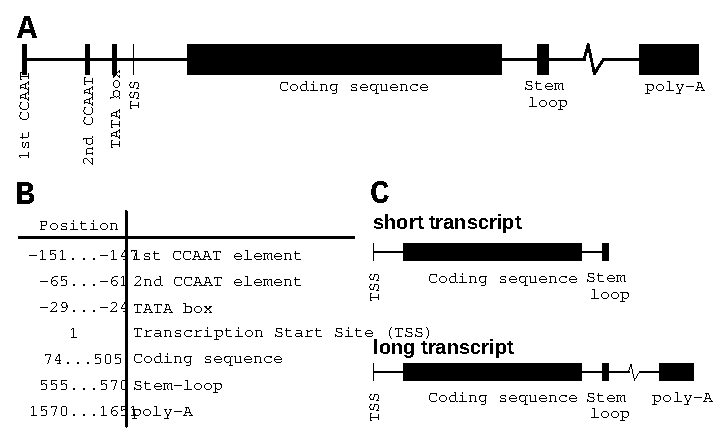
\includegraphics{h2ax-review/figs/Fig2}
\caption[H2AFX gene and transcripts]%
        {H2AFX gene and transcripts. A.~Schematic of H2AFX gene region
          showing promoter and 3' mRNA stabilizing
          elements. B.~Sequence coordinates of each element in H2AFX
          relative to transcription start site\@. C.~Alternative
          transcripts of H2AFX\@. The short transcript
          ($\approx$\SI{600}{\bp} in size) ends in a stem--loop like
          canonical histones, whereas the long transcript
          ($\approx$\SI{1600}{\bp} in size) ends in a poly-(A) tail.}
\label{fig:h2ax-review:H2AFX}
\end{figure}

\subsection{H2AX Transcripts}
A fundamental distinction between histone types is whether their
expression is replication-dependent or replication-independent. This
difference is a consequence of the requirement for large amounts of
canonical histones during S~phase to package the newly duplicated
genome (i.~e.\ replication-dependence).
In contrast, variant or ``replacement'' histones often appear to be
inserted into chromatin to replace canonical histones for functional
reasons throughout the cell cycle and are therefore
replication-independent \citep{Marzluff02}.

Canonical histone genes lack introns, probably to circumvent the
requirement for primary transcript processing when histones must be
rapidly produced at S~phase. A number of transcript features appear to
enhance the capacity of replication-dependent histone expression by up
to 35-fold during S~phase.  In fact, there is only a five-fold
increase in their transcription rate at S phase, compared to the other
phases of cell cycle so regulation acts strongly at the
post-transcriptional level \citep{HarrisMCB1991}.
Replication-dependent histone transcripts lack a poly(A) tail and
encode a stem--loop followed by a purine-rich Histone Downstream
Element (HDE) downstream of the stop codon. The stem--loop interacts
with the Stem--Loop Binding Protein (SLBP) to stabilise the mRNA in
S~phase \citep{SLBP-regulation} while the HDE interacts with U7~snRNA to direct
efficient 3' end processing \citep{HDE-sequence}.

Human H2AX transcripts exhibit characteristics of both
replication-dependent and replication-independent histones. The H2AFX
gene lacks introns, and has two alternative transcripts: one shorter
form contains the characteristic stem--loop, and the other longer form
contains a downstream poly(A) tail \citep{HTwoAX-transcripts}
\frefp{fig:h2ax-review:H2AFX}. The combined synthesis of H2AX
transcripts has been described as ``weakly replication-linked at
best'' since the H2AFX promoter keeps the levels of both transcripts
high through the cell cycle \citep{VSI94}. However, the cell cycle
linkage of the forms is unclear and no study has reported the effect
of DNA damage on transcription levels.

\subsection{H2AX Protein}
\label{subsec:h2ax-review:H2AX-protein}
Despite the large amount of attention paid to the DNA damage-linked
serine phosphorylation by PIKKs, the H2AX protein itself has a number
of additional unique properties.

The defining feature of H2AX is considered to be the C-terminal
region with the SQ[E/D]\textPhi{} motif
\frefp{fig:h2ax-review:H2AX-logo}. As mentioned in
\Sref{subsec:h2ax-review:relation-H2A-H2AX}, the number of residues
separating this motif from the histone fold is variable and claimed to
correlate with the evolutionary complexity of the organism
\citep{CRDP+02}. The residues responsible for this variable spacing
are mainly hydrophilic with a high glycine and proline content
suggesting a flexible, unstructured nature so the basis for the
correlation could be more directly related to a structural constraint
such as the variation in internucleosomal repeat lengths of organisms
which itself shows linkage with evolutionary complexity.

\begin{sidewaysfigure}
\centering
%% The figure is already rotated on the file (at the time we didn't
%% know better) which means that it may be right or wrong depending on
%% whether it falls on an odd or even page.  We need to change the
%% signal of the rotation depending on where it falls.  On the
%% publication, the caption is also on the margin.  Here we exercise
%% editor rights to put the caption on the side as it happens on all
%% other tables and figures of the thesis (also we don't have margins
%% wide enough for captions).

\includegraphics[angle=-90,width=\textheight]{h2ax-review/figs/Fig3}
\raggedleft
\caption[Sequence logo of human canonical H2A isoforms and H2AX]%
                   {Sequence logo of all human canonical H2A isoforms
                     showing differences with H2AX below. The 4
                     residues changes from H2A to H2AX outside the
                     C-terminal region are Gln\,6\,Thr, Thr\,16\,Ser,
                     Asn\,38\,His and Lys\,99\,Gly. Alignment of H2A
                     genes was made usign edialign
                     \citep{Mor99} from EMBOSS
                     \citep{RLB00} and WebLogo 3
                     \citep{weblogo}.}%
\label{fig:h2ax-review:H2AX-logo}
\end{sidewaysfigure}

In addition to the C-terminal motif, amino acid residues 6, 16, 38
and 99 of H2AX are different from the human H2A.1 consensus
(\fref{fig:h2ax-review:H2AX-logo} and
\ref{fig:h2ax-review:H2AInNucleosome}). Inspection of the human and
\species{X.\ laevis} histone based nucleosome structures reveals that
H2A residue~6 is located in the flexible N-terminal tail and
residue~16 is located at the very base of the tail
(\fref{fig:h2ax-review:H2AInNucleosome} and
\ref{fig:h2ax-review:framed:b}) which tracks the minor groove at
superhelical location~4.5 (SHL4.5)
\frefp{fig:h2ax-review:framed:a}. The substitution of glutamine with
threonine at position~6 in H2AX introduces a potential hydroxyl site
for post-translational modification that is not present for the
glutamine in canonical H2A. In contrast, the threonine to serine
substitution conserves the modifiable hydroxyl at position~16.

\begin{figure}
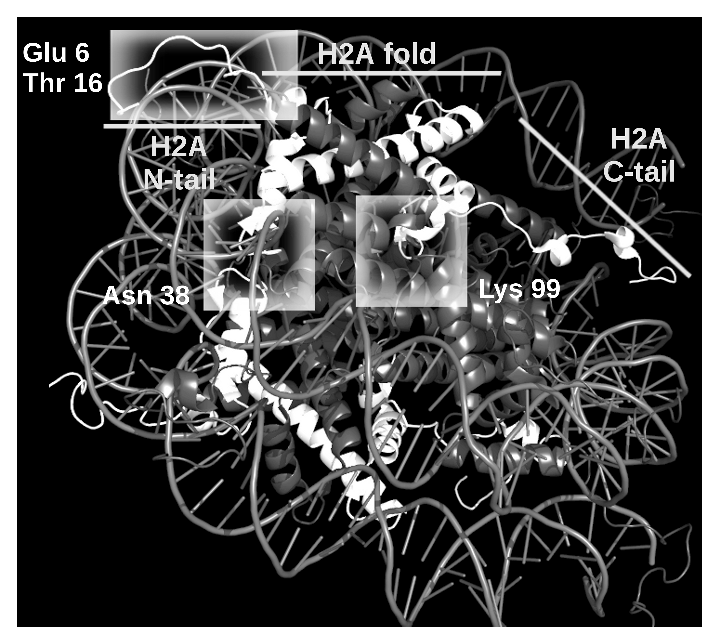
\includegraphics{h2ax-review/figs/Fig4}
\caption[Nucleosome structure highlighting differences between H2A and H2AX]%
        {Nucleosome structure highlighting differences between H2A and
          H2AX\@. H2A chain is highlighted and white frames indicate
          the position of the residues that differ between the human
          canonical H2A and H2AX\@. Image from PDB structure 1KX5
          using PyMOL \citep{DeL02}.}
\label{fig:h2ax-review:H2AInNucleosome}
\end{figure}

\begin{figure}
\centering
\subbottom[]{%
  \includegraphics[width=0.45\textwidth]%
  {"h2ax-review/figs/Fig 5A - H2A Ntail"}
  \label{fig:h2ax-review:framed:a}
}
\subbottom[]{%
  \includegraphics[width=0.45\textwidth]%
  {"h2ax-review/figs/Fig 5B - 6Q + 16T"}
  \label{fig:h2ax-review:framed:b}
}
\subbottom[]{%
  \includegraphics[width=0.45\textwidth]%
  {"h2ax-review/figs/Fig 5C - 38N"}
  \label{fig:h2ax-review:framed:c}
}
\subbottom[]{%
  \includegraphics[width=0.45\textwidth]%
  {"h2ax-review/figs/Fig 5D - 99R"}
  \label{fig:h2ax-review:framed:d}
}

\caption[Structural environment of H2A residues that differ from H2AX]%
        {Structural environment of H2A residues that differ from
          H2AX\@. The van der Waals surface of differences and all
          residues within \SI{5}{\angstrom} are shown as a surface of
          dots over bond sticks. Image from PDB structure 1KX5 using
          PyMOL \citep{DeL02}.
          \subcaptionref{fig:h2ax-review:framed:a}~H2A N-terminal
          tail encompassing H2AX residues Thr\,6 and Ser\,16 passes
          across minor groove at superhelical location (SHL) 4.5\@.
          \subcaptionref{fig:h2ax-review:framed:b}~Closeup of H2A
          N-terminal tail minor groove association from A showing
          canonical H2A Gln\,6 and Thr\,16 which become, respectively,
          Thr\,6 and Ser\,16 in H2AX\@.
          \subcaptionref{fig:h2ax-review:framed:c}~Residues around
          H2A--H2A association in structure showing interaction
          between paired Asn\,38 sidechains and adjacent
          residues. Canonical H2A Asn\,38 is His\,38 in mammalian
          H2AX\@.
          \subcaptionref{fig:h2ax-review:framed:d}~Environment around
          H2A Arg\,99 showing unusual absence of close packing.
          Canonical H2A Arg\,99 is Gly\,99 in H2AX.}
\label{fig:h2ax-review:framed}
\end{figure}

Asparagine~38 is located in the loop between the \textalpha 1 and
\textalpha 2 helices of H2A within the nucleosome
(\fref{fig:h2ax-review:H2AInNucleosome} and
\ref{fig:h2ax-review:framed:c}). Importantly, this residue makes
direct contact with the equivalent amino acid in the other H2A--H2B
dimer in the nucleosome structure and has been suggested to affect
both nucleosome stability and the balance between homotypic and
heterotypic combinations (see
\Sref{subsec:h2ax-review:H2AX-distribution}) of H2A types within the
yeast nucleosome \citep{CLW01}. It is possible that the change of
residue~38 from asparagine in H2A to histidine in H2AX could also
affect nucleosome stability and dynamics. For example, weakening of
interactions between the two H2A-H2B histone fold dimers could result
in increased nucleosome flexing and impact the ability to condense
into stable higher order chromatin structure. Furthermore, the
presence of the histidine in H2AX could affect the stabilisation of a
second copy of H2AX relative to canonical H2A within the
nucleosome. This change of asparagine to histidine at position~38
occurs only in higher organism H2AX and could potentially drive a bias
towards either homotypic H2AX-only or heterotypic H2AX--H2A mixed
nucleosomes which could have consequences for the distribution of H2AX
in chromatin (see \Sref{subsec:h2ax-review:H2AX-distribution}).

The effect of the final substitution distinguishing canonical H2A and
H2AX where lysine becomes glycine at position~99 is less clear. This
residue is located in a sharp turn immediately after the \textalpha 3
helix and points towards the C-terminal ends of H3 and H4 but makes
no direct interactions in the nucleosome
(\fref{fig:h2ax-review:H2AInNucleosome} and
\ref{fig:h2ax-review:framed:d}). Nevertheless, the exchange of the
large, positively charged and potentially modifiable lysine for the
highly flexible glycine in H2AX could potentially alter stability and
flexibility of the nucleosome.

\subsection{H2AX Post-Translational Modifications}
\label{subsec:h2ax-review:H2AX-PTM}
Histones typically have a large proportion of amino acid residues
which are modified post-translationally for functional reasons so it
is significant that three of the four residues distinguishing human
H2A and H2AX in the core region are capable of distinction via
post-translational modification (i.~e.\ Thr\,6 and Ser\,16 in H2AX
vs.\ Thr\,16 and Lys\,99 in canonical H2A).

However, only the phosphorylation of H2AX serine 139 by PIKKs in
response to DNA damage has been intensively studied. This modification
has been demonstrated to enhance access of restriction enzymes and DNA
methylases to the DNA, possibly by reducing nucleosome stability
\citep{KHHK+08}. In the same study the activity of the FACT complex
which can facilitate dissociation of H2A/H2B dimers from nucleosomes
was shown to increase after H2AX phosphorylation.

One of the most recently reported post-translational modifications of
H2AX related to DSB is the phosphorylation of tyrosine~142 in the PIKK
recognition motif of human H2AX \citep{XLS+09,CJT+09}. In contrast to
the phosphorylation of Ser\,139, this Tyr\,142 residue is
phosphorylated under normal conditions with DNA damage acting as
trigger for its dephosphorylation. The dephosphorylation seems to not
only precede the phosphorylation of Ser\,139, but also to be a
prerequisite for the Ser\,139 phosphorylation. When Tyr\,142 is
phosphorylated, affinity of Ser\,139 to the DNA damage response
factors MDC1, MRE11 and Rad50 is greatly reduced and binding by
pro-apoptopic factor JNK1 was found to occur instead. It has therefore
been suggested that the phosphorylation status of Tyr\,142 is a
determinant of cell fate after DNA damage.

H2AX can also be subject of acetylation at lysine~5 \citep{PB81} and
to both mono- and poly-ubiquitylation at lysine~119 dependent on the
prior acetylation at Lys\,5 \trefp{tab:h2ax-review:H2AX-PTM}
\citep{ITK+07}. These modifications are intimately related to DNA
repair because their levels increase significantly after exposure to
DSB-inducing Ionising Radiation (IR) and appear to drive H2AX eviction
from the nucleosome by the action of Tip60 complex and UBC13
\citep{ITK+07}. However, conflicting data about the interdependence of
these effects with phosphorylation has recently been reported
\citep{RVD+09}.

\begin{table}
\centering
\caption[Reported Post-Translational Modifications (PTMs) for H2AX]%
        {Reported Post-Translational Modifications (PTMs) for
          H2AX\@. Other PTMs present in H2A but not yet related to
          H2AX include acetylation of lysine 9 and 13 \citep{ZEP+03},
          phosphorylation of threonine 120 \citep{ANY+04}, and the
          possible methylation of lysine 127 \citep{ZEP+03}.}
\label{tab:h2ax-review:H2AX-PTM}
\begin{tabularx}{\linewidth}{r l l l >{\raggedright\arraybackslash}X}
\toprule
\makecell{Residue\\number} & \makecell{Residue\\indentity} & PTM & \makecell{Related\\to DSB} & Reference  \\
\midrule
1   & Serine & phosphorylation & no  & \citet{PB81} \\
5   & Lysine    & acetylation     & yes & \citet{PB81} and \citet{ITK+07} \\
9   & Lysine    & biotinylation   & no  & \citet{CCK+06} \\
13  & Lysine   & biotinylation   & no  & \citet{CCK+06} \\
119 & Lysine  & ubiquitylation  & yes & \citet{ITK+07} \\
139 & Serine  & phosphorylation & yes & \citet{EPR+98} \\
142 & Tyrosine  & phosphorylation & yes & \citet{XLS+09} \\
\bottomrule
\end{tabularx}
\end{table}

Other modifications unrelated to DNA damage have been reported for
H2AX, including a rather unusual biotinylation of Lys\,9 and Lys\,13
\citep{CCK+06} and the phosphorylation of Ser\,1 \citep{PB81}. By
homology to canonical H2A, it is probable that Lys\,9 and Lys\,13 can
also be acetylated \citep{ZEP+03} and Thr\,120 phosphorylated
\citep{ANY+04}. Another interesting possible post-translational
modification is a methylation at Lys\,127 \citep{ZEP+03}. Although it
was inconclusive whether Lys\,125 or Lys\,127 is the target of this
methylation, it is tempting to speculate that it occurs at Lys\,127
since this residue is the only one conserved in the C-terminal of all
human H2A sequences \frefp{fig:h2ax-review:H2AX-logo}.

\subsection{H2AX Distribution in Chromatin}
\label{subsec:h2ax-review:H2AX-distribution}
The original estimates of H2AX abundance in human cells reported cell
line specific values from \SIrange{2.5}{25}{\percent} of total H2A in
asynchronous immortalised cell lines \citep{EPR+98}. These values were
determined by densitometry of Coomassie-stained, acid-extracted
histones in two-dimensional gels. A \pcent{10} abundance value of H2AX
has become accepted despite wide differences in the study and the fact
that HeLa cells were reported to contain \pcent{2.5} H2AX\@.

Although it is tempting to interpret \pcent{10} abundance as implying
every tenth nucleosome will contain H2AX, combinatorial features of
nucleosomes make the statistics of spacings between H2AX occurrences
in the chromatin fibre more complex. H2AX can be incorporated either
as one or as two copies per nucleosome
(\fref{fig:h2ax-review:H2AX-distribution}A), and the H2AX-containing
nucleosomes can be either randomly or non-randomly distributed along
the chromatin fibre (\fref{fig:h2ax-review:H2AX-distribution}B--C).
Random incorporation would lead not simply to each tenth nucleosome
containing H2AX, but to a geometric distribution of spacings between
H2AX-containing nucleosomes. This predicts many instances of small
spacings and some instances of very large spacings, and has clear
implications for the ability of \textgamma H2AX to signal local damage
events as well as for the spreading of the phosphorylation along the
chromatin fibre.

\begin{figure}
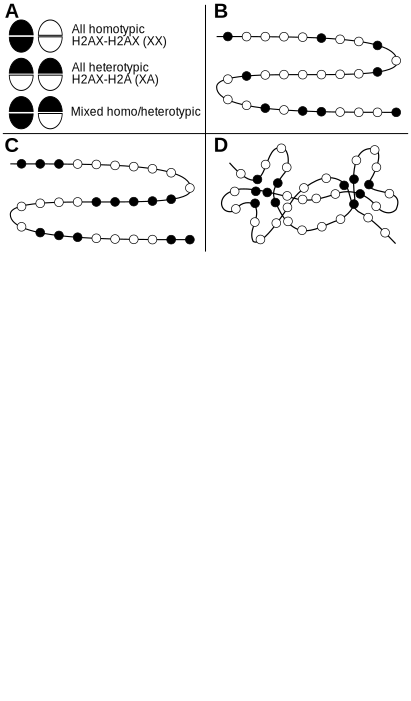
\includegraphics{h2ax-review/figs/Fig6}
\caption[H2AX distribution in the chromatin]%
        {H2AX distribution in the chromatin.
          A.~Schematic of possible H2AX homotypic, heterotypic and
          mixed nucleosome combinations. Black semicircle represents
          H2AX--H2B dimer and white semicircle represents H2A--H2B
          dimer.
          B.~Random incorporation of H2AX into nucleosomes would lead
          to a random distribution of H2AX-containing nucleosomes.
          C.~Selective incorporation of H2AX into nucleosomes would
          lead to ``islands'' of H2AX-containing nucleosomes.
          D.~Random incorporation of H2AX nucleosomes could also lead
          to ``islands'' of H2AX nucleosomes by chromatin
          reorganization.}
\label{fig:h2ax-review:H2AX-distribution}
\end{figure}

\subsubsection{Combinatorial potential in H2AX distribution}
The combinatorial potential for H2AX inclusion has two separate
features which could affect the detailed distribution of H2AX along
chromatin.

Firstly, either one or two H2AX polypeptides can in principle be
present within a nucleosome: Two H2AX copies would give rise to a
``homotypic'' H2AX/H2AX (`XX') nucleosome, whereas a single H2AX copy
will give rise to a ``heterotypic'' H2AX/H2A (`XA') nucleosome
(\fref{fig:h2ax-review:H2AX-distribution}A).
It is currently unknown whether there is a bias for either homotypic
or heterotypic nucleosomes (see
\Sref{subsec:h2ax-review:H2AX-protein}) although this affects the
statistics of H2AX spacing in chromatin since the XA combination
yields twice as many H2AX-containing nucleosomes than XX for a given
H2AX abundance.

Secondly, the spacing of nucleosomes containing H2AX should have a
major influence on its functional roles in DSB signaling, assembling
of repair foci and facilitating the repair machinery. H2AX nucleosomes
could be randomly distributed
(\fref{fig:h2ax-review:H2AX-distribution}B) or subject to clustering
in one (\fref{fig:h2ax-review:H2AX-distribution}C) or three dimensions
(\fref{fig:h2ax-review:H2AX-distribution}D). Any mechanism randomly
assembling chromatin from pools of XX and/or XA versus canonical
H2A--H2A (`AA') nucleosomes will give rise to a geometric distribution
of spacings between H2AX (\fref{fig:h2ax-review:H2AX-graphs}A).
This distribution predicts a bias towards small spacings
(\fref{fig:h2ax-review:H2AX-graphs}A).

\begin{figure}
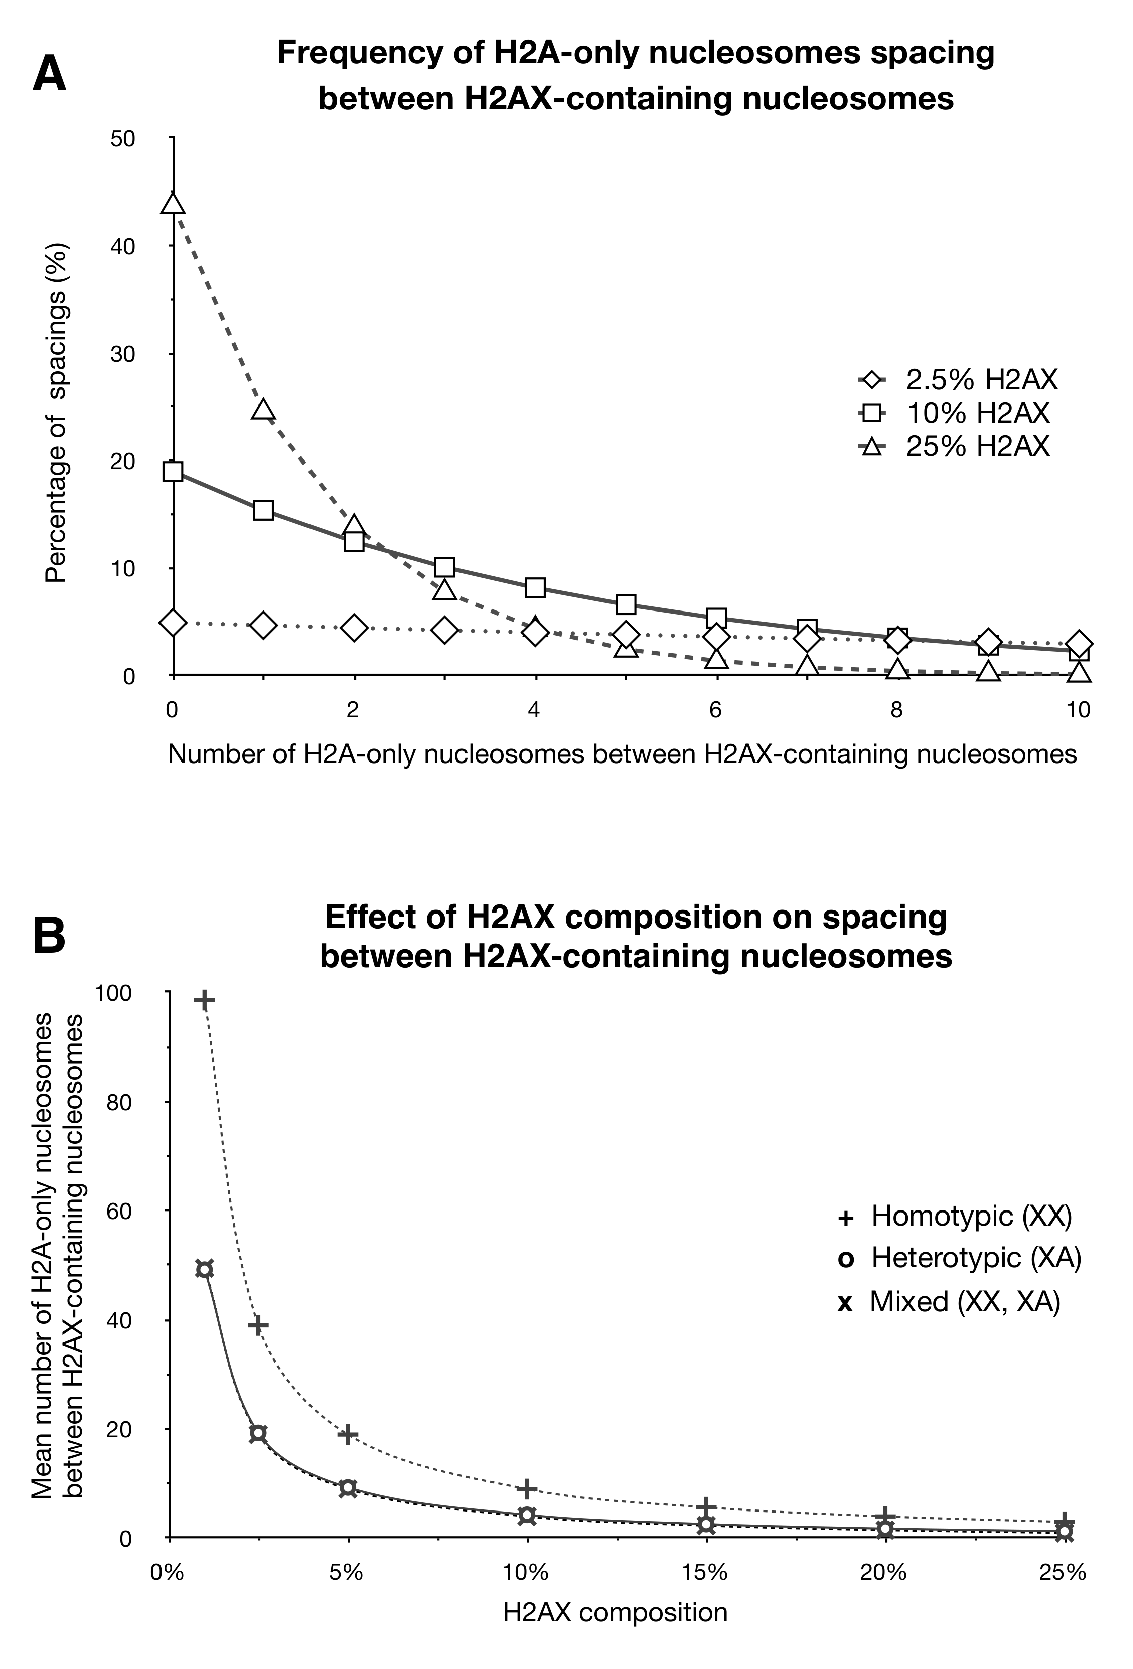
\includegraphics[width=\textwidth]{h2ax-review/figs/Fig7}
\caption[Simulations of H2AX spacing distributions]%
        {Simulations of H2AX spacing distributions.
          A.~Distribution of spacings between instances of H2AX for
          mixed population of homotypic and heterotypic nucleosomes at
          abundances of \pcent{2.5} (dot), \pcent{10} (solid) and
          \pcent{25} (dashed) H2AX in total H2A pool.
          B.~Effect of abundance on mean H2AX spacing for homotypic
          (H2AX--H2AX) only, heterotypic (H2AX--H2A) only, and mixed
          homotypic$+$heterotypic nucleosome combinations.}
\label{fig:h2ax-review:H2AX-graphs}
\end{figure}

\subsubsection{Simulation of random H2AX inclusion}
Simple computational simulations reveal interesting features in this
H2AX spacing distribution. In the simplest case of H2AX assembling in
a mixture of XA and XX nucleosomes, \pcent{10} overall H2AX abundance
would generate an average of 4.3 nucleosomes between H2AX occurrences
along the chromatin fibre (\fref{fig:h2ax-review:H2AX-graphs}B). The
mean spacing is highly sensitive to H2AX abundance
(\fref{fig:h2ax-review:H2AX-graphs}A), so \pcent{2.5} and \pcent{25}
H2AX abundances yields means of 19.3 to 1.3 nucleosomes, respectively
(\fref{fig:h2ax-review:H2AX-graphs}B). Similar results arise for
calculations where only heterotypic XA nucleosomes can assemble and
homotypic XX nucleosomes are structurally precluded. In contrast, if
heterotypic XA nucleosomes are precluded and only XX nucleosome
structures can assemble, then \pcent{10} H2AX abundance yields a mean
spacing of 9 nucleosomes between H2AX occurrences. The mean spacings
for \pcent{2.5} and \pcent{25} H2AX abundance are 39 to 3 nucleosomes
respectively (\fref{fig:h2ax-review:H2AX-graphs}B).

\subsubsection{Functional implications of H2AX distribution}
These simple models of random nucleosome incorporation have
interesting implications. The occurrence of occasional large H2AX
spacings could limit both processive \textgamma H2AX spreading along
the chromatin fibre and the proximity of H2AX in solenoidal higher
order chromatin packaging. At \pcent{10} H2AX abundance, \pcent{23} of
nucleosomes in mixed XA and XX nucleosomes will be spaced by more than
6 nucleosomes and in the extreme case of \pcent{2.5} H2AX abundance,
\pcent{84} of solely homotypic XX nucleosomes would be spaced by more
than 6 nucleosomes.

This sensitivity of H2AX spacing in chromatin to abundance provides a
potential opportunity for the cell to regulate responsiveness to
damage. For example, if H2AX expression is up-regulated the mean
proximity of randomly inserted H2AX will rapidly increase and effects
such as processive \textgamma H2AX spreading and retention of DDR
factors at foci will be significantly enhanced.

It is unknown whether H2AX distribution varies between euchromatin and
heterochromatin. However, differences in H2AX response have been
reported according to the condensation level of chromatin and
phosphorylation of Ser\,139 has been observed to occur preferentially
in euchromatin \citep{IGC+07}.
This preference is overcome during replication of heterochromatin when
it is in a less condensed state \citep{IGC+07}. The distinction
between active and inactive chromatin can also be regulated, as
demonstrated for phosphorylation of KAP-1 by ATM reducing the access
of DNA repair proteins to heterochromatic regions of the genome
\citep{AAG+08}.

\subsubsection{Possibility of non-random H2AX distribution}
If H2AX nucleosome incorporation is not a random process
(\fref{fig:h2ax-review:H2AX-distribution}B), inhomogeneity could also
exist at a more local level. For example, small ``islands'' of higher
density H2AX nucleosomes could be interspersed within broader regions
with lower relative abundance of the variant
(\fref{fig:h2ax-review:H2AX-distribution}C). A recent study using a
novel high-resolution microscopy observed several thousand small
spatial clusterings of H2AX and pointed to a mutual exclusivity of
H2AX and the phosphorylated form \citep{JBBTB06}. This would be
consistent with a clustering model
(\fref{fig:h2ax-review:H2AX-distribution}D) that enhanced the kinetics
of the damage signaling at foci, perhaps by making use of a chromatin
structural feature such as the chromosomal scaffold
\citep{JBBTB06}. The inherent clustering and active insertion of H2AX
in the DDR could also drive larger scale chromosomal rearrangements
through chromatin stability
(\fref{fig:h2ax-review:H2AX-distribution}D) \citep{KHHK+08}.

\section{Functional Roles of H2AX}
Phosphorylation of H2AX serine 139 by PIKKs to generate ``\textgamma
H2AX foci'' is an early and characteristic feature of DSB events. This
modification is thought to be the primary identifier of the location
of DNA damage and would therefore be central to the function of H2AX.

The \textgamma H2AX foci extend for \SIrange{2}{30}{\mega\bp} along
the chromatin fibre \citep{EPR+99}, implying the involvement of a span
of \numrange{e4}{e5} nucleosomes per individual DSB repair event. At
\pcent{10} H2AX abundance, this would involve up to \numrange{e2}{e4}
H2AX molecules and hence a \numrange{e2}{e4} fold amplification of DSB
event signal. A direct link between the site of a lesion and a single
focus has been observed \citep{KRIK+03}, suggesting that there is a
linkage between \textgamma H2AX and the repair mechanism. Many protein
factors have been identified, which depend directly or indirectly on
the phosphorylation of H2AX at serine 139. Thereafter, it appears to
act as a foundation for recruitment of DDR factors at DSB sites
\citep{TTP+00}. As a consequence, H2AX performs a role in both
localisation and structuring of the repair focus.

\subsection{Initiation of H2AX Phosphorylation as a Reporter of DSB Events}
The process of establishing H2AX phosphorylation at the characteristic
terminal motif can be performed by any of the three PIKKs ATM, ATR and
DNA-PK\@. Their induction and binding characteristics suggest that
H2AX phosphorylation for focus generation can be distinguished by an
initiation phase when a small number of phosphorylations are made at
nucleosomes adjacent to the break, and a spreading phase in which a
larger region of phosphorylation extends one-dimensionally from either
side of the break.
The structural exposure of the serine 139 site through chromatin
flexibility will be crucial determinant of the modification event (see
\Sref{subsec:h2ax-review:H2AX-PTM}).

ATM has been considered a strong candidate as the principal kinase
responsible for the initiation phase of general damage events because
it responds to changes in chromatin conformation expected when a
spontaneous DSB event releases local superhelical tension
\citep{CJB03}. ATR appears to be linked to replication stress or UV
damage events which lead to breaks as indirect consequences, so ATR is
recruited by ATRIP which detects single-stranded DNA\@. DNA-PK is
localised to DSBs in complex with the end-binding protein Ku, so such
an association will act to limit the distance from the damaged end on
which DNA-PK can act \citep{WCG01} and such an end-dependent
mechanism would be sensitive to H2AX abundance and distribution.

\subsection{Spreading of H2AX Phosphorylation as a Damage Signal Amplifier}
The conventional model for \textgamma H2AX focus formation suggests
that after initiation in the immediate vicinity of the break by ATM
and/or DNA-PK, amplification occurs by spreading through the action
of MDC1 binding to \textgamma H2AX \citep{MSJAC+05}. MDC1 in turn
recruits the MRN complex (Mre11--Rad50--Nbs1) via direct interaction
with Nbs1 \citep{LMS+04} and the MRN complex further activates ATM
\citep{ULM+03}. This generates a positive feedback loop to drive
spreading of the phosphorylation modification away from the
break. Hence H2AX acts both as signal and target of phosphorylation in
the spreading phase. Each focus acts independently even when several
foci are formed in the immediate vicinity of each other
\citep{MJK+06}, suggesting a one dimensional diffusion along the
chromatin fibre.

How the signal spreads over megabase but non-infinite distances is
unknown. It is possible that non-homogeneous H2AX distribution could
contribute to the localisation of \textgamma H2AX stochastically
through random occurrence of large spacings between H2AX that the
spreading mechanism could not bridge (see
\Sref{subsec:h2ax-review:H2AX-distribution}). Consistent with this,
high resolution microscopy reveals that H2AX is not randomly
distributed but organized into discrete clusters which would control
the expansion of the signal \citep{JBBTB06}.

Since levels of phosphorylated H2AX rise rapidly in response to damage
and then reduce over time \citep{EPR+98} it is necessary to remove
either the phosphate or the entire \textgamma H2AX\@. The timing of
this process is unclear but must depend on the presence of \textgamma
H2AX binding factors such as MDC1 which could stabilise \textgamma
H2AX or obscure the phosphate group \citep{MSJAC+05}. In
\species{S.\ cerevisiae}, dephosphorylation is achieved by removal of
phosphorylated H2AX from nucleosomes and subsequent dephosphorylation
by the HTP-C complex \citep{MKJK+06}. In higher eukaryotes the
mechanisms remain unclear since several phosphatases have been
implicated in the process and these can variously dephosphorylate H2AX
within nucleosomes or after removal \citep{CKI+05,KTA+06,CXZ+08}. In
addition, the FACT complex which facilitates nucleosome exchange has
enhanced activity on phosphorylated H2AX \citep{KHHK+08} suggesting at
least one pathway involving displacement for extra-nucleosomal
dephosphorylation. A background level of H2AX remains phosphorylated
even in the apparent absence of DNA damage, but the reason for this is
unknown \citep{EPR+98}.

\subsection{\textgamma H2AX and Chromatin Structural Remodelling}
Intrinsically, H2AX phosphorylation must take place within the context
of chromatin structure so both the Non-Homologous End Joining (NHEJ)
and Homologous Recombination (HR) pathways can efficiently undertake
DSB repair. To facilitate this, chromatin decondenses near the DSB
\citep{MJK+06} but the mechanism for this remodeling is unclear.

The modified serine 139 of H2AX is located near the DNA entry/exit
point on the nucleosome \frefp{fig:h2ax-review:H2AInNucleosome} so
one putative mechanism for the chromatin structural change is to be
driven directly by the chemical properties of the added phosphate
group. \species{S.\ cerevisiae} mutants with the serine 139 equivalent
mutated to glutamate to mimic the phosphate charge show increased
micrococcal nuclease sensitivity consistent with such a
destabilisation \citep{JAD00} and phosphorylated human H2AX renders
chromatin more susceptible to restriction enzymes and DNA methylase
\citep{KHHK+08}. However, a separate analysis of chromatin structure,
also in yeast, harboring the glutamate mutation did not find evidence
of direct chromatin structural effects \citep{FIT07}.

An alternative indirect mechanism for linking H2AX phosphorylation
with chromatin disruption is by recruitment of proteins to drive
remodeling. A number of different ATP-dependent chromatin remodeling
activities have been implicated in this process, including RSC,
SWI/SNF, INO80 and SWR (reviewed in \citet{JAD07}), as well as other
nucleosome modifying enzymes such as the NuA4 histone
acetyltransferase. There is also evidence that chromatin chaperones
and binding proteins contribute to the process of chromatin dynamics
at DSBs. For example, the FACT complex, which participates in exchange
between H2A and H2AX, has greater ability to mobilise \textgamma H2AX
than unphosphorylated H2AX \citep{KHHK+08}. In addition, HP1\textbeta,
which binds to H3~K9me, has recently been shown to be released by
phosphorylation immediately after DSB events and that this contributes
to H2AX phosphorylation by PIKKs \citep{AJB+08}.

Both direct and indirect mechanisms for chromatin remodeling depend on
H2AX phosphorylation, and hence require an independent initiation
step. The PIKKs ATM and DNA-PK can achieve this by detecting changes
in chromatin structure or appearance of DNA ends, respectively
\citep{CJB03,BC04}.
However, the impact of chromatin on PIKK initiation is difficult to
probe because H2AX phosphorylation occurs very rapidly after DSBs,
making it difficult to temporally distinguish factors which remodel
chromatin to enable initial PIKK access from downstream events which
undertake remodeling to amplify \textgamma H2AX around the site.

Furthermore, despite the intimate link between H2AX phosphorylation
and chromatin remodeling at the DSB site, local decondensation of
chromatin occurs at similar levels on both wild type and H2AX$^{-/-}$
cell lines when ATP is not depleted \citep{MJK+06}. This suggests that
the role of H2AX phosphorylation in driving the chromatin remodeling
is redundant with other pathways.

\subsection{\textgamma H2AX and Localisation of DSB Repair Proteins}
Since H2AX phosphorylation is one of the earliest events after a DSB,
this suggests it may play a role in subsequent recruitment of the
active repair proteins. This is supported by the absence of RAD51 and
BRCA1 at DSB foci when \textgamma H2AX phosphorylation is prevented
\citep{TTP+00}. However, NBS1, BRCA1 and 53BP1 are recruited to the
sites of damage in H2AX$^{-/-}$ cell lines which display only moderate
sensitivity to ionising radiation but fail to maintain focal
localisation \citep{ACOF+03}.
It has therefore been suggested that the crucial role of H2AX
phosphorylation is not as a direct agent of repair factor recruitment,
but of retention of these factors in the vicinity of the DSB
\citep{ACOF+03}.
This role in defining a ``damage neighborhood'' does not necessarily
imply a direct role in repair at the break site itself. For example,
stimulation of the G2/M checkpoint may result from the accumulation of
checkpoint signalling factors at the focus \citep{OFHC+02}. In fact,
Chromatin ImmunoPrecipitation (ChIP) revealed that \textgamma H2AX is
evicted from the region close to the DSB early in the DDR in
\species{S.\ cerevisiae} and that \textgamma H2AX does not strictly
co-localise with the active repair complexes \citep{RSAA+04}.

This accumulated retention of DDR factors in the vicinity of a DSB
appears to be a complex process where the initiating damage signal is
integrated by factors recognising the H2AX phosphorylation and
presumably additional chromatin features. For example, human 53BP1 and
its putative homologues, \species{S.\ cerevisiae} Rad9 and
\species{S. pombe} Crb2, all contain Tudor domains which bind specific
methylated histones in chromatin, and BRCT domains which can both
mediate dimerisation and bind \textgamma H2AX\@. Despite the
similarity in domain structure of Rad9, Crb2 and 53BP1, individual
investigations have indicated that they have different binding
capabilities. The Rad9 Tudor domain binds H3~K79me
\citep{GCJ+07,HZDJ+04} whereas Crb2 and 53BP1 Tudor domains bind
H4~K20me2 \citep{SPM+04,BLW+06}.  Rad9 and Crb2 BRCT domains bind
directly to \textgamma H2AX \citep{HMH+07,KDR+08} whereas 53BP1 does
not, instead relying on an indirect interaction mediated by the BRCT
domain of MDC1 which directly binds \textgamma H2AX
\citep{MSL+05,MSJAC+05}. Some direct interaction between 53BP1 BRCT
domain and \textgamma H2AX has also been reported by co-precipitation
studies, but in a much smaller proportion than Rad9 and Crb2
\citep{KDR+08}. Rad9 and Crb2 can all also dimerise or oligomerise
through their BRCT domains \citep{SL99,DMR04} although this domain is
not necessary for the oligomerisation of 53BP1 \citep{AWX+05}. The
latter instead requires a sequence upstream of its Tudor domain
\citep{WKM+06}.

This complex interplay between the combinatorial interactions made by
53BP1, Rad9 and Crb2 with themselves and with \textgamma H2AX builds
up to generate another level of the structural environment for the
repair process. \textgamma H2AX therefore acts as a foundation to
define the extent of the repair focus through the H2AX distribution
and the extent of its phosphorylation.

\subsection{\textgamma H2AX and Maintenance of Proximity of Break Ends}
Linked to this role in retaining repair factors in the repair focus,
phosphorylated H2AX also appears to function in the bringing together
of damaged ends. It has been suggested that by recruiting repair
factors which directly associate with the damaged ends, H2AX could
prevent diffusion of these ends away from each other \citep{BA04}. For
example, linkage has been observed in the distribution of cohesin and
\textgamma H2AX near DSBs \citep{UAS+04} so \textgamma H2AX-dependent
cohesin association would promote the stabilisation of sister
chromatids to facilitate HR\@. Furthermore, localisation of
self-interacting factors by their association with \textgamma H2AX
nucleosomes could bring together distant break ends. For example,
53BP1 is suggested to localise to break ends by direct interaction
with nucleosomes and indirect interaction through MDC1
\citep{HZDJ+04,BLW+06,EAR+09}. Oligomerisation of 53BP1 has also been
reported to enhance association of distant ends, thereby facilitating
long range recombination and NHEJ \citep{DGW+08,DCS+08}.

\subsection{\textgamma H2AX and Complementary Damage Signalling Via Ubiquitylation}
A secondary pathway of signaling by ubiquitylation of both canonical
H2A and H2AX has recently been uncovered which appears to derive
directly from \textgamma H2AX, and therefore act as a complementary
amplification of the damage signal \citep{PD09}. Recognition of H2AX
phosphorylation by MDC1 leads to recruitment of an initiating
ubiquitylation by RNF8 and UBC13 which is subsequently amplified with
the involvement of RNF158, and possibly maintained by Rap80 and
BRCT1\@. The direct role of the ubiquitylation remains to be clarified
because it can act in factor recruitment as well as affecting the
structure, stability or turnover of histones including H2AX itself.

\section{Conclusion}
Despite H2AX having a highly similar primary sequence or even
overlapping identity with canonical H2A, it is clear that the DNA
damage-linked function of this histone variant is highly specific. Its
functional role is as an amplifier of the damage event signal, a
foundation for marshaling repair factors, and a promoter of the
chromatin dynamics required to complete the repair process. It is
clear that the phosphorylation of serine 139 by PIKKs generates an
epitope which is crucial to these functions. Nevertheless, it is
important to note that the DNA damage response is only moderately
defective in H2AX$^{-/-}$ cells, suggesting that complementary
mechanisms must operate redundantly with H2AX functions. Much remains
to be appreciated about \textgamma H2AX structure and function, but
this must ultimately be based on the unique distinguishing features of
the H2AX gene and protein.

\subsubsection*{Acknowledgements}
We thank Prof.\ Cathal Seoighe for assistance with calculations of
random H2AX distribution, Prof.\ Noel Lowndes for his input and
Dr.\ Kevin Roche for helpful discussions. We gratefully acknowledge
the support of Science Foundation Ireland and Health Research Board of
Ireland for supporting work in our laboratory. DMSP acknowledges the
support of the Portuguese Foundation for Science and Technology (FCT).
